\documentclass[12pt]{article}
\usepackage[margin=1in]{geometry}
\usepackage{textcomp}
\usepackage{multirow}
\usepackage{graphicx}
\pagestyle{empty}

\setlength{\parskip}{\baselineskip}
\setlength{\parindent}{0pt}

\begin{document}
\begin{center}
\large Control Rod Worth Calibration \\
\normalsize Generated \today
\end{center}

\emph{Control rod worths}

\begin{tabular}{r c}
	Safe Rod & \textbf{%(safeworth)s} \\
	Shim Rod & \textbf{%(shimworth)s} \\
	Reg Rod & \textbf{%(regworth)s} \\ \hline
	Total & \textbf{%(totalworth)s}
\end{tabular}

\emph{Peak reactivity addition rates for each control rod}

\begin{tabular}{r c c c c}
	& Max.\ Add.\ Rate & Max.\ Add.\ Rate & Spec & OK? \\
	Safe & \textbf{%(safemaxdpp)s} & \textbf{%(safemaxdps)s} & $< 12$ \textcentoldstyle/sec & \textbf{%(safedpsok)s} \\
	Shim & \textbf{%(shimmaxdpp)s} & \textbf{%(shimmaxdps)s} & $< 12$ \textcentoldstyle/sec & \textbf{%(shimdpsok)s} \\
	Reg & \textbf{%(regmaxdpp)s} & \textbf{%(regmaxdps)s} & $< 12$ \textcentoldstyle/sec & \textbf{%(regdpsok)s}
\end{tabular}

Plots of the original data, and polynomials of best fit, are on the next page.

\emph{Core excess and shutdown margin}

The core excess is calculated twice: once using the Safe Rod at its lowest critical point with the other two rods removed, and once using the Shim Rod in the same configuration. Both values of the CXS are given here; they should be nearly equal.

The shutdown margin and one-stuck-rod SDM are also calculated using each value of the CXS. For the ``one stuck rod'' rule, we assume that the most reactive control rod, in this case the \textbf{%(mostrxvrod)s}, is completely withdrawn.

\begin{tabular}{r c c c c}
	& Safe & Shim & Spec & OK? \\
	CXS height & \textbf{%(safecxsht)s} & \textbf{%(shimcxsht)s} & --- & --- \\
	Core excess & \textbf{%(safecxs)s} & \textbf{%(shimcxs)s} & $< \$3.00$ & \textbf{%(cxsok)s} \\
	Shutdown margin & \textbf{%(safesdm)s} & \textbf{%(shimsdm)s} & $> \$1.00$ & \textbf{%(sdmok)s} \\
	One-stuck-rod SDM & \textbf{%(safeosr)s} & \textbf{%(shimosr)s} & $> \$0.50$ & \textbf{%(osrok)s}
\end{tabular}

\begin{tabular}{c c c}
	\underline{\hspace{3in}} & {\Large /} & \underline{\hspace{1in}} \\
	Operator Signature & & Date
\end{tabular}

\newpage
\newgeometry{margin=0.5in}
\begin{center}
    \begin{tabular}{c c}
    \multicolumn{2}{c}{\textbf{Safe Rod}} \\
    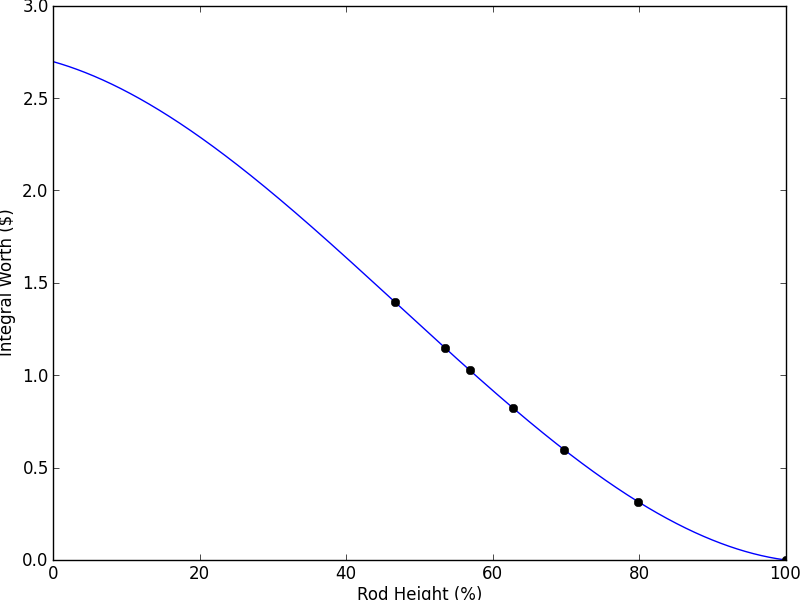
\includegraphics[width=3.2in]{safe-integral} & 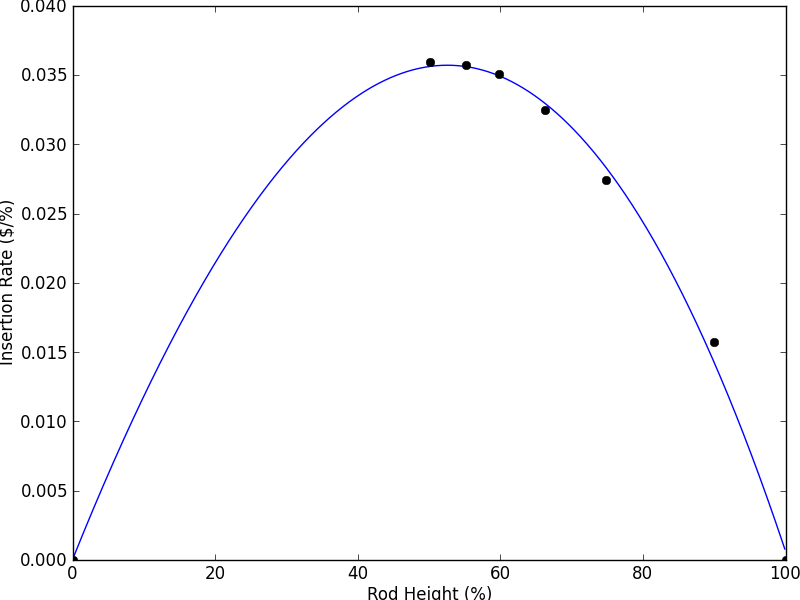
\includegraphics[width=3.2in]{safe-rate} \\
    \multicolumn{2}{c}{\textbf{Shim Rod}} \\
    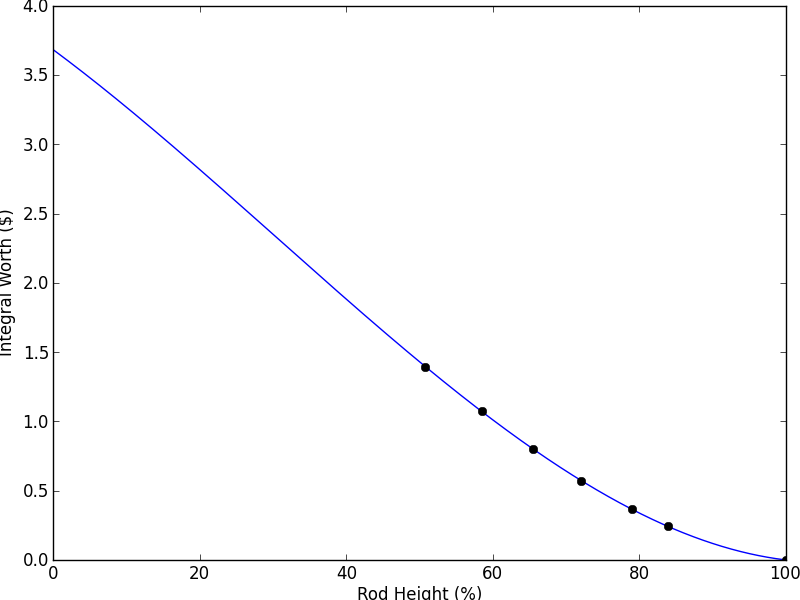
\includegraphics[width=3.2in]{shim-integral} & 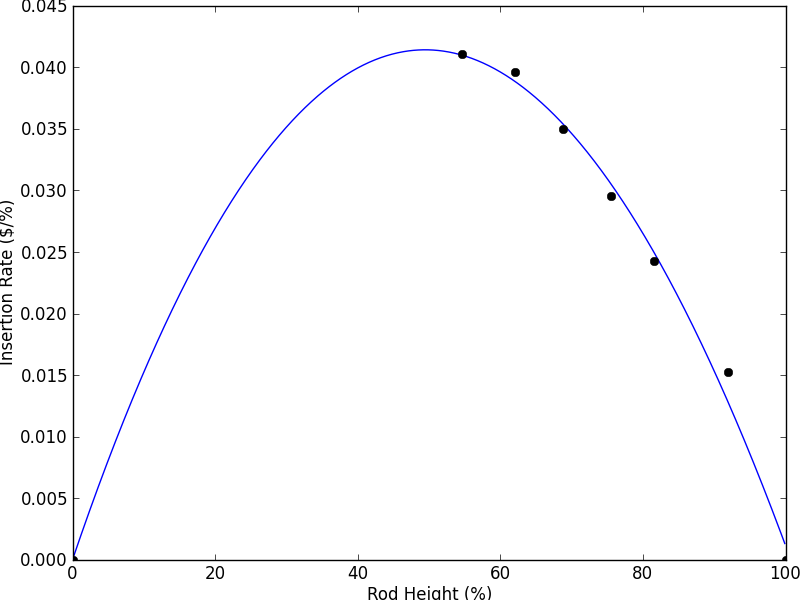
\includegraphics[width=3.2in]{shim-rate} \\
    \multicolumn{2}{c}{\textbf{Reg Rod}} \\
    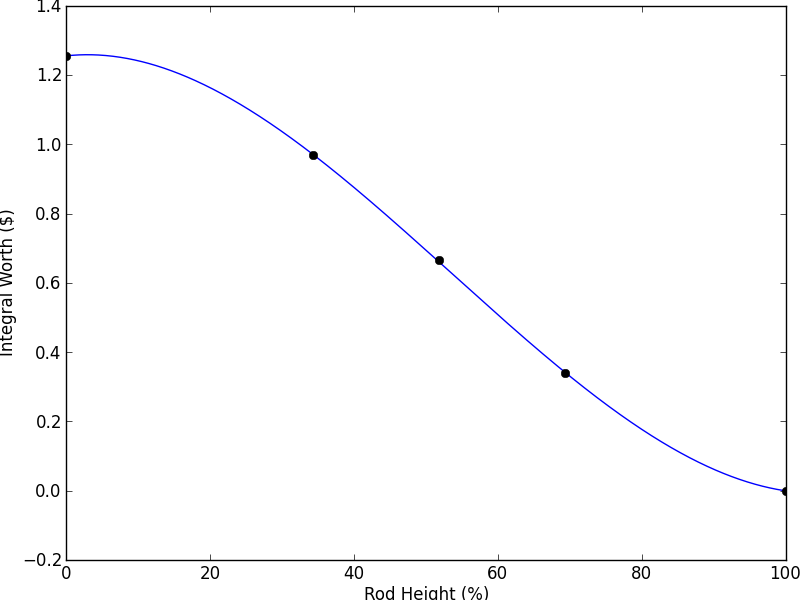
\includegraphics[width=3.2in]{reg-integral} & 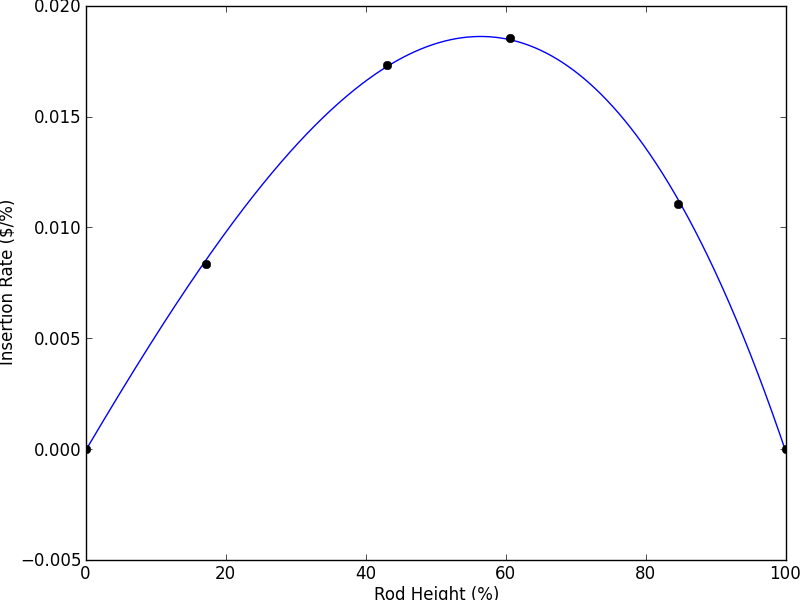
\includegraphics[width=3.2in]{reg-rate} \\
    \end{tabular}
\end{center}

\begin{tabular}{r l}
Safe Int. Worth: & %(safeintpoly)s \\
Safe Add. Rate:  & %(safeaddpoly)s \\
Shim Int. Worth: & %(shimintpoly)s \\
Shim Add. Rate:  & %(shimaddpoly)s \\
Reg Int. Worth:  & %(regintpoly)s \\
Reg Add. Rate:   & %(regaddpoly)s \\
\end{tabular}
\end{document}
